\section{Results}
\label{measurement:results}

This section presents the results of carrying out the methodology described in
Section~\ref{measurement:methodology} to the Alexa 10k, including measurements
of the popularity distribution of \JS features with and without blocking, a
feature's popularity in relation to its age, and which features are frequently
blocked.


\subsection{Definitions}
This Chapter uses the term \textbf{feature popularity} to
denote the percentage of sites that use the feature at least once during
automated interaction with the site.  A feature that is used on every site has
a popularity of 1, and a feature that is never seen has a popularity of 0.

Similarly, the term \textbf{standard popularity} denotes the
percentage of sites that use at least one feature from the standard at least
once during the site's execution.

Finally, we use the term \textbf{block rate} to denote how frequently a feature
would have been used if not for the presence of an advertisement- or
tracking-blocking extension. Browser features that are used much less
frequently on the web when a user has AdBlock Plus or Ghostery installed have
high block rates. Features that are used on roughly the same number of
websites in the presence of blocking extensions have low block rate.


\subsection{Standard Popularity}
This subsection presents measurements of the popularity of the standards in the
browser, first in general, then followed by comparisons to the individual
features in each standard, the popularity of sites using each standard, and
when the standard was implemented in \FF.


\subsubsection{Overall}

\begin{figure}[ht]
  \centering
  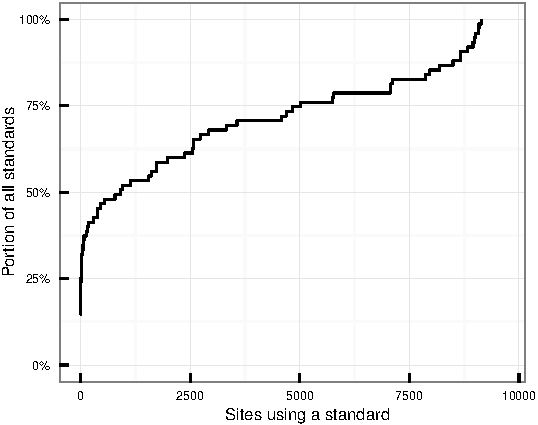
\includegraphics[width=.5\textwidth]{figures/feature_popularity.pdf}
  \caption{Cumulative distribution of standard popularity within the Alexa 10k.}
  \label{fig:popcdf}
\end{figure}

Figure~\ref{fig:popcdf} displays the cumulative distribution of standard
popularity. Some standards are extremely popular, others are extremely
unpopular: six standards are used on over 90\% of all websites measured, while
28 of the 75 standards measured were used on 1\% or fewer sites;
eleven are not used at all. The remaining standards saw intermediate
popularity levels.


\subsubsection{Standard Popularity By Feature}
Browser features are not equally used on the web.  Some features are extremely
popular, such as the \texttt{Document.prototype.createElement} method,
used to create new page-elements.  The feature is used on 9,079--or over
90\%--of pages in the Alexa 10k.

Other browser features are never used.  689 features, or almost 50\% of the
measured \numfeatures, were never observed on the 10k most popular
sites.  A further 416 features are used on less than 1\% of the 10k most
popular websites.  Put together, this means that over 79\% of the features
available in the browser are used by less than 1\% of the web.

Browser features also do not have equal block rates. Some features
are blocked by advertisement and tracking blocking extensions far more often
than others.  Ten percent of browser features are prevented from executing over
90\% of the time when browsing with common blocking extensions.   We also find
that 1,159 features, or over 83\% of features available in the browser, are
executed on less than 1\% of websites in the presence of popular advertising
and tracking blocking extensions.


\subsection{Standard Popularity vs. Site Popularity}
\label{measurement:results:popularity}

\begin{figure}[th]
  \centering
  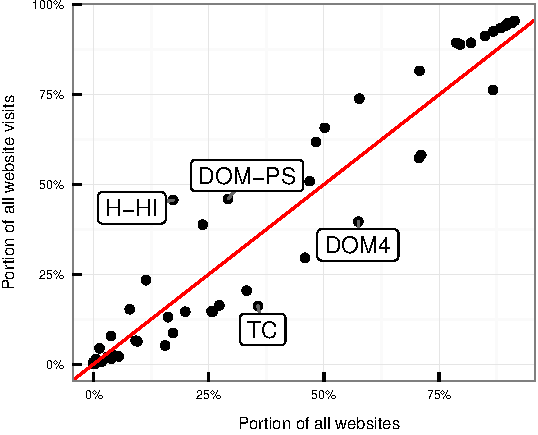
\includegraphics[width=.5\textwidth]{figures/sites_vs_visits_scatter.pdf}
  \caption{Comparison of percentage of sites using a standard versus percentage of web traffic using a standard.}
  \label{fig:feature-pop-by-site-pop}
\end{figure}


Most of the results presented in this Section give equal weight to all sites in
the Alexa 10k.  Put differently, if the most popular and least popular sites use the same
standard, both uses are given equal consideration.  This Section considers
the difference between the number of sites using a standard, and the
percentage of site visits using a standard.

Figure \ref{fig:feature-pop-by-site-pop} presents this comparison.
The x-axis shows the percentage of sites that use at least one feature from a
standard, and the y-axis shows the estimated percentage of site views on the
web that use this standard.  Standards above the \texttt{x=y} line are more
popular on frequently visited sites, meaning that the percentage of page views
using the standard is greater than the percentage of sites using the standard.
A site on the \texttt{x=y} line indicates that the feature is used exactly as
frequently on popular sites as on less popular sites.

Generally, the graph shows that standard usage is not equally distributed, and
that some standards are more popular with frequently visited sites.  However,
the general trend appears to be for standards to cluster around the
\texttt{x=y} line, indicating that while there are some differences in standard
usage between popular and less popular sites, they do not appear to be
substantial.

Therefore, for the sake of brevity and simplicity, all other measures in this
paper treat standard use on all domains as equal, and do not consider a site's
popularity.

In addition to the datasets used in this paper, we have also collected data
from even-less popular sites from the Alexa one-million (sites with rank less
than 10k, to determine whether the less-popular websites seem to use different
features than popular websites.  We found no significant, notable difference
between these two groups.  The rest of this work, therefor, as a simplifying
assumption, treats the Alexa 10k as representative of the web in general.


\subsection{Standard Popularity By Introduction Date}
\begin{figure}[ht]
  \centering
  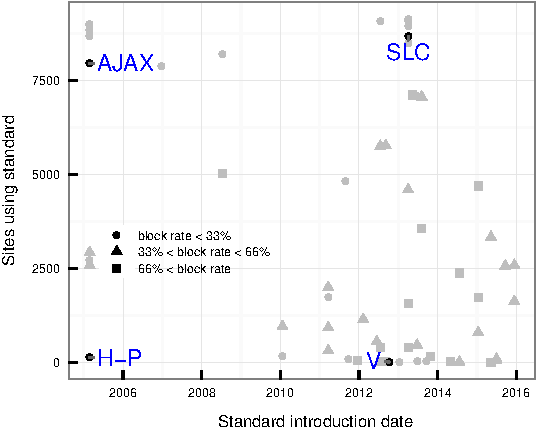
\includegraphics[width=.5\textwidth]{figures/date_popularity.pdf}
  \caption{Comparison of a standard's availability date, and its popularity.}
  \label{fig:date_popularity}
\end{figure}


We also measured the relationship between when a standard became available in
the browser, its popularity, and how frequently its execution is prevented by
popular blocking extensions.

As the graph shows, there is no simple relationship between when a standard was
added to the browser, how frequently the standard is used on the web, and how
frequently the standard is blocked by common blocking extensions.  However, as
\ref{fig:date_popularity} indicates, some standards have become extremely
popular over time, while others, both recent and old, have languished in
disuse. Furthermore, it appears that some standards have been introduced
extremely recently but have nevertheless been readily adopted by web authors.

\subsubsubsection{Old, Popular Standards} For example, point \textbf{AJAX}
depicts the \textit{XMLHttpRequest}~\cite{ajaxwhatwg}, or \textit{AJAX} standard,
used to send information to a server without fetching the entire document
again.  This standard has been available in the browser for almost as long as
\FF has been released (since 2004), and is extremely popular. The standard's
most popular feature, \texttt{XMLHttpRequest.prototype.open}, is used by 7,955
sites in the Alexa 10k.  Standards in this portion of the graph have been in
the browser for a long time, and appear on a large fraction of sites.  This
cluster of standards have block rates of less than 50\%, considered low in this
study.

\subsubsubsection{Old, Unpopular Standards}
Other standards, despite existing in the browser nearly since \FF's inception,
are much less popular on the web.  Point \textbf{H-P} shows the \textit{HTML:
Plugins}~\cite{htmlpluginsw3c} standard, a subsection of the larger \textit{HTML}
standard that allows document authors to detect the names and capabilities of
plugins installed in the browser (such as Flash, Shockwave, Silverlight, etc.).
The most popular features of this standard have been available in \FF since
2005.  However, the standard's most popular feature,
\texttt{PluginArray.prototype.refresh}, which checks for changes in browser
plugins, is used on less than 1\% of current websites (90 sites).

\subsubsubsection{New, Popular Standards}
Point \textbf{SEL} depicts the \emph{Selectors API Level
1}~\cite{selectors1w3c} standard, which provides site authors with a simplified
interface for selecting elements in a document.  Despite being a relatively
recent addition to the browser (the standard was added in 2013), the most
popular feature in the
standard--\texttt{Document.prototype.querySelectorAll}--is used on over 80\% of
websites.  This standard, and other standards in this area of the graph, have
low block rates.

\subsubsubsection{New, Unpopular Standards}
Point \textbf{V} shows the \textit{Vibration}~\cite{vibrationapi} standard,
which allows site authors to trigger a vibration in the user's device on
platforms that support it.  Despite this standard having been available in \FF
longer than the previously mentioned \textit{Selectors API Level 1} standard,
the \textit{Vibration} standard is significantly less popular on the web.  The
sole method in the standard, \texttt{Navigator.prototype.vibrate}, is used only
once in the Alexa 10k.


\subsection{Standard Blocking}
\label{sec:results-feature-blocking}
Many users alter their browsing environment when visiting websites.  They do so
for a variety of reasons, including wishing to limit advertising displayed on
the pages they read, reducing their exposure to malware distributed through
advertising networks, and increasing their privacy by reducing the amount of
tracking they experience online.  These browser modifications are commonly
made by installing browser extensions.

The following Sub-Sections present the effect of installing two common browser
extensions, AdBlock Plus and Ghostery, on the type and number of features that
are executed when visiting websites.

\subsubsection{Popularity vs. Blocking}
\label{sec:results-feature-popularity}

\begin{figure}[ht]
  \centering
  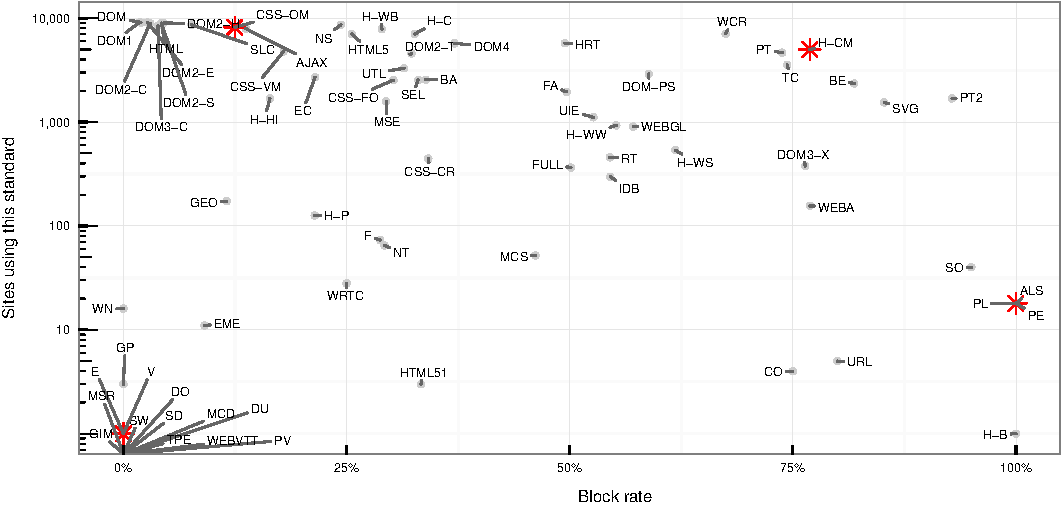
\includegraphics[width=\textwidth]{figures/megagraph.pdf}
  \caption{Popularity of standards versus their block rate, on a log scale.}
  \label{fig:megagraph}
\end{figure}


Ad and tracking blocking extensions do not block the use of all standards
equally.  Figure \ref{fig:megagraph} shows the relationship between a
standard's popularity (represented by the number of sites the standard was used
on, log scale) and its block rate.  Recall that this work measures a standard's
popularity as the number of sites where a feature in a standard is used at
least once.  Therefor, the popularity of the standard is equal to at least the
popularity of the most popular feature in the standard.

Each quadrant of the graph tells a different story about the popularity and the
block rate of a standard on the web.

\subsubsubsection{Popular, Unblocked Standards} The upper-left quadrant
contains the standards that occur very frequently on the web, and are rarely
blocked by advertising and tracking blocking extensions.

One example, point \textbf{CSS-OM}, depicts the \textit{CSS Object
Model}~\cite{cssomw3c} standard, which allows \JS code to introspect, modify
and add to the styling rules in the document.  It is positioned near the top of
the graph because 8,193 sites used a feature from the standard at least once
during measurement.  The standard is positioned to the left of the graph
because the standard has a low block rate (12.6\%), meaning that the addition
of blocking extensions had relatively little effect on how frequently sites
used any feature from the standard.

\subsubsubsection{Popular, Blocked Standards} The upper-right quadrant of the
graph shows standards that are used by a large percentage of sites on the web,
but which blocking extensions frequently prevent from executing.

A representative example of such a standard is the \textit{HTML: Channel
Messaging} ~\cite{htmlcmw3c} standard, represented by point \textbf{H-CM}.
This standard contains \JS methods allowing embedded documents
(\texttt{iframes}) and windows to communicate with their parent document.  This
functionality is often used by embedded-content and pop-up windows to
communicate with the hosting page, often in the context of advertising.  This
standard is used on over half of all sites by default, but is prevented from
being executed over 77\% of the time in the presence of blocking extensions.

\subsubsubsection{Unpopular, Blocked Standards} The lower-right quadrant of the
graph shows standards that are rarely used by websites, and that are almost
always prevented from executing by blocking extensions.

Point \textbf{ALS} shows the \emph{Ambient Light Events}
standard~\cite{ambientlightapi}, which defines events and methods allowing a
website to react to changes to the level of light the computer, laptop or
mobile phone is exposed to.  The standard is rarely used on the web (14 out of
10k sites), but is prevented from being executed 100\% of the time by blocking
extensions.

\subsubsubsection{Unpopular, Unblocked Standards} The lower-left quadrant of
the graph shows standards that were rarely seen in our study, and were rarely
prevented from executing.  Point \textbf{E} shows the
\emph{Encodings}~\cite{encodingw3c} standard.  This standard allows \JS code to
read and convert text between different text encodings, such as reading text
from a document encoded in \emph{GBK} and inserting it into a website encoded
in \emph{UTF-8}.

The \emph{Encodings}~\cite{encodingw3c} standard is rarely used on the web,
with only 1 of the Alexa 10k sites attempting to use it.  However, the addition
of an advertising or tracking blocking extension had no affect on the number of
times the standard was used; this sole site still used the \emph{Encodings}
standard when AdBlock Plus and Ghostery were installed.


\subsubsection{Blocking Frequency}
As discussed in \ref{sec:results-feature-popularity}, blocking extensions do
not block all browser standard usage equally; as Figure \ref{fig:megagraph}
shows, some standards are greatly impacted by installing these advertising and
tracking blocking extensions, while others are not impacted at all.

For example, the \textit{Beacon}~\cite{beaconapi} standard, which allows
websites to trigger functionality when a user leaves a page, has a 83.6\%
reduction in usage when browsing with blocking extensions.  Similarly, the
\emph{SVG} standard, which includes functionality that allows for
fingerprinting users through font enumeration\footnote{The
\texttt{SVGTextContentElement.prototype.getComputedTextLength} method}, sees a
similar 86.8\% reduction in site usage when browsing with blocking extensions.

Other browser standards, such as the core \textit{DOM} standards, see little
reduction in use in the presence of blocking extensions.


\subsubsection{Blocking Purpose}
\begin{figure}[ht]
  \centering
  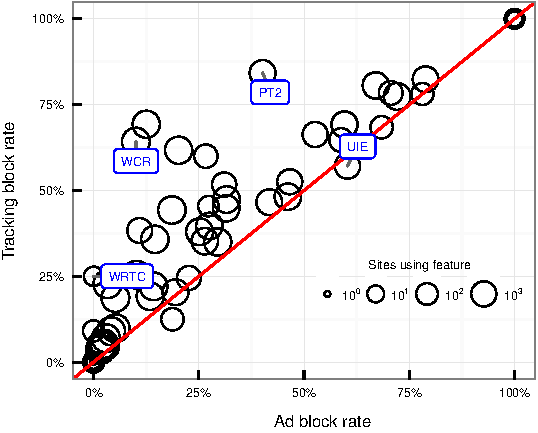
\includegraphics[width=.5\textwidth]{figures/ad_vs_tracking_blocking.pdf}
  \caption{Comparison of block rates of standards using advertising vs. tracking blocking extensions.}
  \label{fig:feature-blocking-source}
\end{figure}


In addition to measuring which standards were blocked by extensions, we also
distinguished \emph{which} extension did the blocking.
Figure~\ref{fig:feature-blocking-source} plots standards' block rates in the
presence of an advertising blocking extension (x-axis), versus standards' block
rates when a tracking-blocking extension is installed (y-axis).

Points on the \texttt{x=y} line in the graph are standards that were blocked
equally in the two cases, with points closer to the upper-right corner being
blocked more often (in general), and points closer to the lower-left corner
being blocked less often (in general).

Points in the upper-left depict standards that were blocked more frequently by
the tracking-blocking extension than the advertising-blocking extension, while
points in the lower-right show standards that were blocked more frequently by
the advertising-blocking extension.

As the graph shows, some standards, such as \emph{WebRTC}~\cite{webrtcw3c}
(which is associated with attacks revealing the user's IP address),
\emph{WebCrypto API}~\cite{webcryptow3c} (which is used by some analytics
libraries to generate identifying nonces), and \emph{Performance Timeline Level
2}~\cite{perftimingw3c} (which is used to generate high resolution time stamps)
are blocked by tracking-blocking extensions more often than they are blocked by
advertisement blocking extensions.

The opposite is true, to a lesser extent, for the \emph{UI Events
Specification}~\cite{uievents3c} standard, which specifies new ways that sites
can respond to user interactions.
